%%%%%%%%%%%%%%%%%%%%%%%%%%%%%%%%%%%%%%%%%
% Programming/Coding Assignment
% LaTeX Template
%
% This template has been downloaded from:
% http://www.latextemplates.com
%
% Original author:
% Ted Pavlic (http://www.tedpavlic.com)
%
% Note:
% The \lipsum[#] commands throughout this template generate dummy text
% to fill the template out. These commands should all be removed when 
% writing assignment content.
%
% This template uses a Perl script as an example snippet of code, most other
% languages are also usable. Configure them in the "CODE INCLUSION 
% CONFIGURATION" section.
%
%%%%%%%%%%%%%%%%%%%%%%%%%%%%%%%%%%%%%%%%%

%----------------------------------------------------------------------------------------
%	PACKAGES AND OTHER DOCUMENT CONFIGURATIONS
%----------------------------------------------------------------------------------------

\documentclass[a4paper]{article}

\usepackage{fancyhdr} % Required for custom headers
\usepackage{lastpage} % Required to determine the last page for the footer
\usepackage{extramarks} % Required for headers and footers
\usepackage[usenames,dvipsnames]{color} % Required for custom colors
\usepackage{graphicx} % Required to insert images
\usepackage{listings} % Required for insertion of code
\renewcommand*{\lstlistingname}{代码} % change "Listing <ref> to 代码 <ref>
\usepackage{courier} % Required for the courier font
\usepackage{lipsum} % Used for inserting dummy 'Lorem ipsum' text into the template

\usepackage[UTF8]{ctex} % Required for Chinese character
\usepackage{tocloft} % Required for beautiful toc
\usepackage[hidelinks]{hyperref} % Required for clickable toc
\hypersetup{
    colorlinks,
    citecolor=black,
    filecolor=black,
    linkcolor=black,
    urlcolor=black
}
\usepackage[title]{appendix} % Required for appendix
\usepackage{float}
\usepackage{amsmath} % used for \text{} in math formula


% used for beautiful table
\usepackage{booktabs} 
\usepackage[T1]{fontenc}
\usepackage{tabu}
\usepackage{longtable}
\usepackage[table]{xcolor}


% Margins
\topmargin=-0.45in
\evensidemargin=0in
\oddsidemargin=0in
\textwidth=6.5in
\textheight=9.0in
\headsep=0.25in

\linespread{1.1} % Line spacing

% Set up the header and footer
\pagestyle{fancy}
\lhead{\hmwkAuthorName} % Top left header
\chead{\hmwkClass\ (\hmwkClassInstructor\ \hmwkClassTime): \hmwkTitle} % Top center head
\rhead{\firstxmark} % Top right header
\lfoot{\lastxmark} % Bottom left footer
\cfoot{} % Bottom center footer
\rfoot{Page\ \thepage\ of\ \protect\pageref{LastPage}} % Bottom right footer
\renewcommand\headrulewidth{0.4pt} % Size of the header rule
\renewcommand\footrulewidth{0.4pt} % Size of the footer rule

\setlength\parindent{0pt} % Removes all indentation from paragraphs

%----------------------------------------------------------------------------------------
%	CODE INCLUSION CONFIGURATION
%----------------------------------------------------------------------------------------

\definecolor{MyDarkGreen}{rgb}{0.0,0.4,0.0} % This is the color used for comments
\lstloadlanguages{c} % Load Perl syntax for listings, for a list of other languages supported see: ftp://ftp.tex.ac.uk/tex-archive/macros/latex/contrib/listings/listings.pdf
\lstset{language=c, % Use Perl in this example
        frame=single, % Single frame around code
        basicstyle=\small\ttfamily, % Use small true type font
        keywordstyle=[1]\color{Blue}\bf, % Perl functions bold and blue
        keywordstyle=[2]\color{Purple}, % Perl function arguments purple
        keywordstyle=[3]\color{Blue}\underbar, % Custom functions underlined and blue
        identifierstyle=, % Nothing special about identifiers                                         
        commentstyle=\usefont{T1}{pcr}{m}{sl}\color{MyDarkGreen}\small, % Comments small dark green courier font
        stringstyle=\color{Purple}, % Strings are purple
        showstringspaces=false, % Don't put marks in string spaces
        tabsize=4, % 5 spaces per tab
        %
        % Put standard Perl functions not included in the default language here
        % morekeywords={rand},
        morekeywords = [1]{uint16_t, uint32_t, uint8_t, int16_t, int8_t, int32_t}
        %
        % Put Perl function parameters here
        morekeywords=[2]{on, off, interp, __attribute__},
        %
        % Put user defined functions here
        morekeywords=[3]{test},
       	%
        morecomment=[l][\color{Blue}]{...}, % Line continuation (...) like blue comment
        numbers=left, % Line numbers on left
        firstnumber=1, % Line numbers start with line 1
        numberstyle=\tiny\color{Blue}, % Line numbers are blue and small
        stepnumber=2, % Line numbers go in steps of 5,
        firstnumber=1
}

% define C style
\definecolor{main-color}{rgb}{0.6627, 0.7176, 0.7764}
\definecolor{back-color}{rgb}{0.1686, 0.1686, 0.1686}
\definecolor{string-color}{rgb}{0.3333, 0.5254, 0.345}
\definecolor{key-color}{rgb}{0.8, 0.47, 0.196}
\lstdefinestyle{mystyle}
{
    language = C++,
    basicstyle = {\small\ttfamily},
    stringstyle = {\color{Mahogany}},
    keywordstyle = {\color{blue}},
    keywordstyle = [2]{\color{Mahogany}},
    keywordstyle = [3]{\color{blue}},
    keywordstyle = [4]{\color{blue}},
    otherkeywords = {__attribute__,<<,>>,++},
    morekeywords = [2]{__attribute__},
    morekeywords = [3]{<<, >>},
    morekeywords = [4]{++, uint16_t, uint32_t, uint8_t, \#define},
}


% Creates a new command to include a perl script, the first parameter is the filename of the script (without .pl), the second parameter is the caption

\newcommand{\shfilescript}[3]{
\begin{itemize}
\item[]\lstinputlisting[caption=#2, label=lst:#1, language=sh]{#3}
\end{itemize}
}
\newcommand{\shscript}[3]{
\begin{itemize}
\item[]\begin{lstlisting}[label=lst:#1, caption=#2] #3 \end{lstlisting}
\end{itemize}
}

%----------------------------------------------------------------------------------------
%	DOCUMENT STRUCTURE COMMANDS
%	Skip this unless you know what you're doing
%----------------------------------------------------------------------------------------

% Header and footer for when a page split occurs within a problem environment
\newcommand{\enterProblemHeader}[1]{
\nobreak\extramarks{#1}{#1 见下页\ldots}\nobreak{} 
\nobreak\extramarks{接上页}{#1 见下页\ldots}\nobreak{}
}

% Header and footer for when a page split occurs between problem environments
\newcommand{\exitProblemHeader}[1]{
\nobreak\extramarks{接上页}{#1 见下页\ldots}\nobreak{}
\nobreak\extramarks{#1}{}\nobreak{}
}
% TODO:code here enable the number before section, but it disable the numbering of problems
%\setcounter{secnumdepth}{0} % Removes default section numbers
\newcounter{homeworkProblemCounter} % Creates a counter to keep track of the number of problems

\newcommand{\homeworkProblemName}{}

\newenvironment{homeworkProblem}[1][Problem \arabic{homeworkProblemCounter}]{ % Makes a new environment called homeworkProblem which takes 1 argument (custom name) but the default is "Problem #"
\stepcounter{homeworkProblemCounter} % Increase counter for number of problems
\renewcommand{\homeworkProblemName}{#1} % Assign \homeworkProblemName the name of the problem
\section{\homeworkProblemName} % Make a section in the document with the custom problem count
\enterProblemHeader{\homeworkProblemName} % Header and footer within the environment
}{
\exitProblemHeader{\homeworkProblemName} % Header and footer after the environment
}

\newcommand{\problemAnswer}[1]{ % Defines the problem answer command with the content as the only argument
\noindent\framebox[\columnwidth][c]{\begin{minipage}{0.98\columnwidth}#1\end{minipage}} % Makes the box around the problem answer and puts the content inside
}

\newcommand{\homeworkSectionName}{}
\newenvironment{homeworkSection}[1]{ % New environment for sections within homework problems, takes 1 argument - the name of the section
\renewcommand{\homeworkSectionName}{#1} % Assign \homeworkSectionName to the name of the section from the environment argument
\subsection{\homeworkSectionName} % Make a subsection with the custom name of the subsection
\enterProblemHeader{\homeworkProblemName\ [\homeworkSectionName]} % Header and footer within the environment
}{
\enterProblemHeader{\homeworkProblemName} % Header and footer after the environment
}


\newcommand{\codev}[1]{\textsf{#1}}
%----------------------------------------------------------------------------------------
%	NAME AND CLASS SECTION
%----------------------------------------------------------------------------------------

% table color
\definecolor{tableHeader}{RGB}{245, 245, 245}
\definecolor{tableLineOne}{RGB}{245, 245, 245}
\definecolor{tableLineTwo}{RGB}{224, 224, 224}
\newcommand{\tableHeaderStyle}{
    \rowfont{\leavevmode\color{white}\bfseries}
    \rowcolor{tableHeader}
}

%----------------------------------------------------------------------------------------

\newcommand{\hmwkTitle}{操作系统原理实验\ \#5(v2)(保护模式)} % Assignment title
\newcommand{\hmwkDueDate}{Sunday,\ June\ 17,\ 2018} % Due date
\newcommand{\hmwkClass}{16级计科\ 7班} % Course/class
\newcommand{\hmwkClassTime}{周一9-10节} % Class/lecture time
\newcommand{\hmwkClassInstructor}{凌应标} % Teacher/lecturer
\newcommand{\hmwkAuthorName}{颜彬} % Your name
\newcommand{\hmwkAuthorId}{16337269} % Your id 

%----------------------------------------------------------------------------------------
%	TITLE PAGE
%----------------------------------------------------------------------------------------

\usepackage{titling}

\title{
\vspace{2in}
\textmd{\textbf{\hmwkClass:\ \hmwkTitle}}\\
\normalsize\vspace{0.1in}\small{Due\ on\ \hmwkDueDate}\\
\vspace{0.1in}\large{\textit{\hmwkClassInstructor\ \hmwkClassTime}}
\vspace{3in}
}

\author{\textbf{\LARGE{\hmwkAuthorName}} \\ \\ \textbf{\LARGE{\hmwkAuthorId}}}
\date{} % Insert date here if you want it to appear below your name
%----------------------------------------------------------------------------------------

\begin{document}
% \begin{titlingpage} % This is for ignore page number in first page. package titling

\maketitle

%----------------------------------------------------------------------------------------
%	TABLE OF CONTENTS
%----------------------------------------------------------------------------------------

% \setcounter{tocdepth}{2} % Uncomment this line if you don't want subsections listed in the ToC
% set depth in toc

% \renewcommand{\cftsecleader}{\cftdotfill{\cftdotsep}} % used for dots between <section> and <page>

\renewcommand{\contentsname}{Content} % force the word to be "content
\newpage
\tableofcontents
\addtocontents{toc}{~\hfill\textbf{Page}\par}
\newpage

% below are document body


% To have just one problem per page, simply put a \clearpage after each problem
\section{实验目的}
学习中断机制知识,掌握中断处理程序设计的要求。
设计一个汇编程序,实现时钟中断处理程序。
扩展 MyOS4 ,增加时钟中断服务,利用时钟中断实现与时间有关的操作和实现简单的系统调用。 \\ 

进入保护模式,了解进入保护模式的方式,了解保护模式与实模式的不同之处。体会“保护”二字的含义。

\section{实验过程}
    本实验的代码参考了Linus实现的GNU/Linux0.11版本的实现。在看懂其代码的基础上,模仿其实现,
    并在必要的地方修改、删除原代码,并增添自己的代码。以此方式重写和完成了实验五。成功地实现了
    系统调用,触发了时钟中断。
    \subsection{引导程序}
    系统的最前面是boot/boot.s。它由BIOS读到内存的0x7C00处,当它被执行时就会把自己移动到内存的0x90000
    处,并把设备中后2KB字节的代码读到内存的0x90200处。内核的其他部分被读到0x10000处。

    
    如图\ref{fig:boot_address}所示,图片展示了在引导过程中,系统的各个部分在内存中的位置。boot.s程序负责将
    自己移动到0x9000(从1到2),再将操作系统在磁盘的部分载入到内存中(从2到3)。setup.s程序负责读取并存储与机器
    相关的信息,将system模块移动到起始地址为0x00000处(4到5),并作一系列操作以进入保护模式。boot.s不直接将
    system载入到内存中0x00000中,这是由于boot.s还依赖于BIOS中断。BIOS中断的中断向量表还在0x00000处,覆写会
    发生错误。最后程序的控制权交给system模块(5到6)。system模块即为内核的主体部分。\\ 

    值得注意的是,本项目的实现采用宏内核的方式。所有的文件将会链接到一起,成为一个较大的.bin文件。该文件即是本
    system文件。system文件的开头部分被固定地设置为``head.s文件编译后得到的二进制代码'',这是为了确保从setup.s模块
    跳转到system模块(绝对跳转)时,能执行到我们想要执行的代码。通过在链接时加上简单的链接命令,即可让head.s始终
    位于system的头部,这也是head.s文件如此命名的原因。
    \begin{figure}
        \begin{center}
        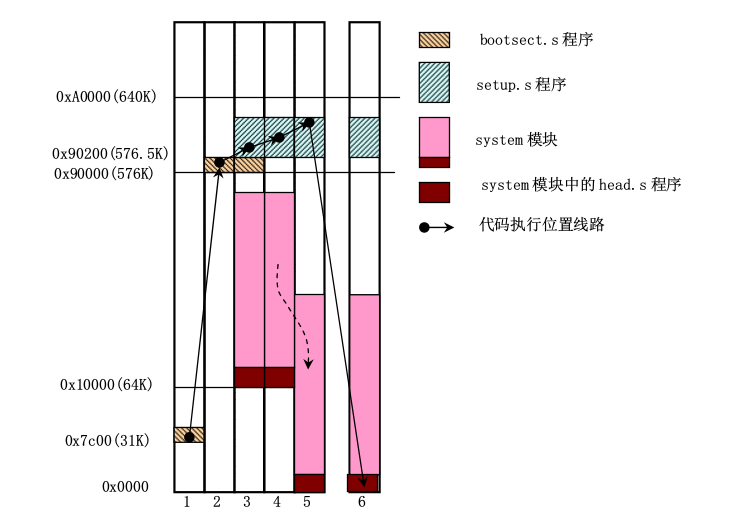
\includegraphics[scale=0.6]{assets/boot_address.png}
        \caption{内核引导过程中的地址变化\label{fig:boot_address}} 
        \end{center} 
    \end{figure} 
    

    \subsection{进入保护模式}\label{sec:pm}
        进入保护模式一般需要一下步骤。加载idt和gdt,开启A20地址线,设置CPU的控制寄存器CR0中的PE位,执行一个跳转
        ,并最终进入保护模式中运行。\\ 
        setup.s程序完成了以上的所有事项,它还重新设置了两个中断控制芯片8259A,将硬件中断号重新设置为0x20-0x2f.\\ 

        \subsubsection{加载gdt}
        描述符见图\ref{fig:segment}所示。由于历史遗留问题,基地址、段界限等内容在描述符中被分开存放。基地址和段界限
        刻画了段的起点和长度。对段外的访问都会出发常规保护错误。可读可写位描述了段的读写权限。一般数据段可读可写,
        代码段只可读,不可写。违反了访问权限,也会触发常规保护错误。\\ 

        指令ldgt使用内存中的一个6字节操作数来加载GDTR寄存器。前两字节用于表示描述符的长度,后4个字节是描述符的基地址。\\

        选择子的作用是指定一个描述符。选择子的低3位用于指令请求特权级(RPL)和访问的是GDT还是LDT(TI)。高13位用于
        指定描述符的索引。\\ 

        一般程序中GDT至少需要3个表项。GDT表的第一项是空项,当使用这个表项访问内存时,会产生一个异常。这个特性可以避免
        陷入意外的引用。剩下的第二和第三个表项分别是代码段和数据段。代码段需要提供只写的保护权限,而数据段需要提供读和
        写的保护权限。\\ 

        \begin{figure}
        \begin{itemize}
        \item[] \begin{lstlisting}[language={[x86masm]Assempler}, label=lst:gdtidt, caption=GDT和IDT]
GDT:
    dw 0, 0, 0, 0 ;dummy

    ; code descriptor
    dw 0x07FF ; limit
    dw 0x0000 ; base address = 0
    dw 0x9A00 ; code, read and exec
    dw 0x00C0 

    ; data descriptor
    dw 0x07FF 
    dw 0x0000 ; base address = 0
    dw 0x9200 ; data, read and write
    dw 0x00C0
idt_48:
    dw 0, 0, 0
gdt_48:
    dw 0x800
    dw 512+GDT, 0x9


        
        \end{lstlisting}
        \end{itemize}
        \end{figure}

        
        \begin{figure}
            \begin{center}
            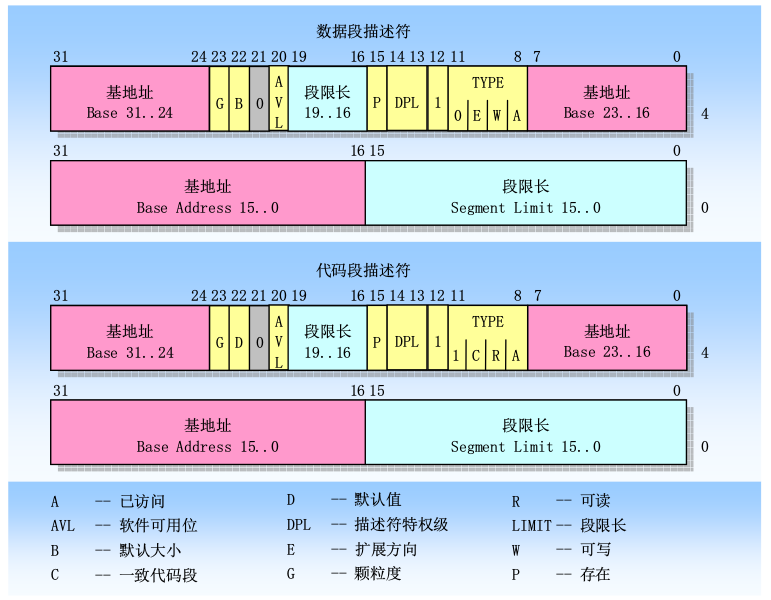
\includegraphics[scale=0.6]{assets/segment.png}
            \caption{代码段和数据段描述符格式\label{fig:segment}} 
            \end{center} 
        \end{figure} 
        

    \subsection{恢复上下文}\label{sec:load}
    \subsection{内存分配模型}
\section{实验结果}
\section{实验总结}
    \subsection{实验心得}
\begin{appendices}
\section{参考文献} \label{sec:reference}
\begin{enumerate}
    \item https://blog.csdn.net/longintchar/article/details/50602851 \\
    16位和32位汇编指令的不同(尤其是push指令)
    \item https://www.ibiblio.org/gferg/ldp/GCC-Inline-Assembly-HOWTO.html\#s1 \\
    GCC 内嵌汇编的书写。
  \end{enumerate}
\end{appendices}
\end{document}
